\chapter{Reinforcement Learning and Genetic Algorithms}
\label{chp:back_RLGA}

This chapter presents the minimal theoretical background of reinforcement learning and genetic algorithms. A particular focus is given to the \ac{PPO} algorithm, which is the main algorithm used in the \ac{RL} framework of the codesign process. Finally, some novel approaches in the field of \ac{RL} are presented. This chapter are based on the work of \citep{sutton_reinforcement_1998,li_deep_2018,agarwal_deep_2022}

\section{Fundamentals of Reinforcement Learning}

Reinforcement learning comes from a fusion of optimal control theory and the theory of machine learning and consists of guiding agents in dynamic environments to maximize cumulative rewards. Unlike supervised learning, \ac{RL} doesn't require labeled input/output pairs, and it focuses on striking a balance between exploring uncharted territory and exploiting existing knowledge. The environment is often modeled as a Markov decision process, distinguishing it from classical dynamic programming by its ability to handle large \ac{MDP}s without assuming an exact mathematical model.

Reinforcement learning's versatility extends to a wide range of disciplines like game theory, control theory, and swarm intelligence. Contrary to optimal control theory's emphasis on exact solutions, \ac{RL} addresses problems without a known mathematical model. Assessing an agent's performance against an optimally acting agent introduces the concept of regret, a measure from decision theory of the disparity between what the agent achieves and the best possible outcome, prompting a deeper understanding of the effectiveness and improvement potential within the learning process. For that, \ac{RL} excels in scenarios involving a trade-off between long-term and short-term rewards, requiring agents to consider the extended consequences of their actions. Overall, its adaptability makes it a powerful tool for complex problems that are difficult to model mathematically, such as multibody dynamics.

\begin{figure}
    \centering
    \caption{Reinforcement Learning Framework}
    \label{fig:rlframework}
    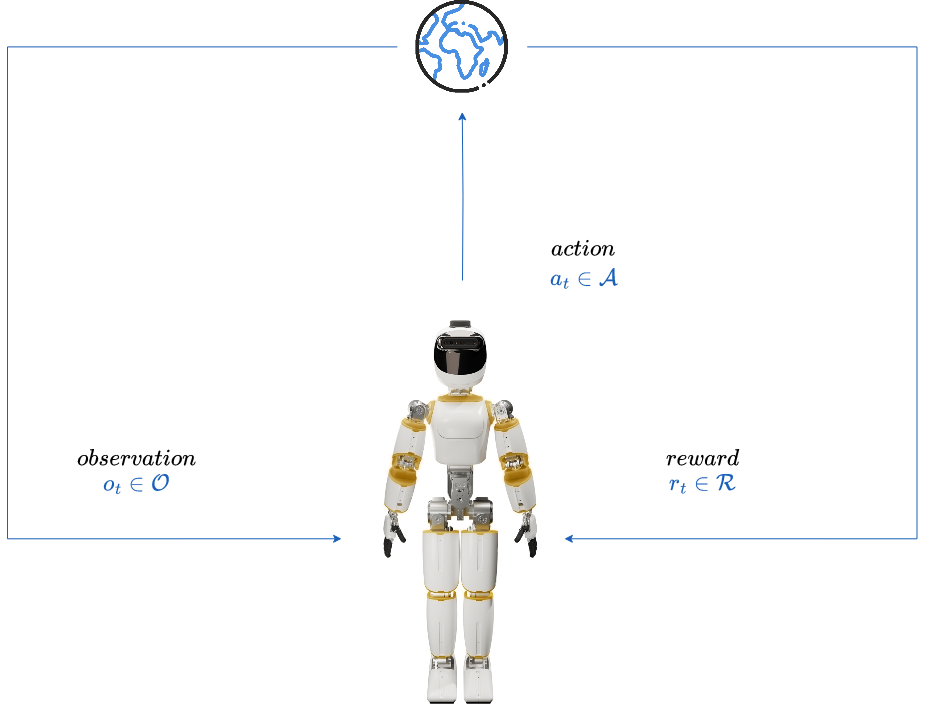
\includegraphics[width=.7\textwidth]{Images/rl_ergocub.png}
\end{figure}

\paragraph{Markov Decision Process} A \ac{MDP} is defined as a five-tuple $\mathcal{M} = (\mathcal{S}, \mathcal{A}, \mathcal{F}, r, \gamma)$ where:

\begin{itemize}
    \item $\mathcal{S}$ is the set of environment states $\mathbf{s} \in \mathcal{S}$, which may be either discrete or continuous
    \item $\mathcal{A}$ is the set of agent actions $\mathbf{a} \in \mathcal{A}$ which in a similar fashion may be continuous or discrete
    \item $\mathcal{F} (\mathbf{s}^\prime | \mathbf{s}, \mathbf{a}): \mathcal{S} \times \mathcal{A} \times \mathcal{S} \rightarrow \mathcal{S}$ is the state-transition function space that describes a conditional probability distribution $\mathcal{F}(\mathbf{s} _{t+1}|\mathbf{s}_t, \mathbf{a} _t)$ that describes the dynamics of the system
    \item $\mathcal{R} (\mathbf{s}^\prime, \mathbf{a}, \mathbf{s}): \mathcal{S} \times \mathcal{A} \times \mathcal{S} \rightarrow \mathbb{R}$ is the reward function
    \item $\gamma \in [0,1]$ is the discount factor that determines the weight of future rewards
\end{itemize}

If the environment is \textit{deterministic}, state transitions can be expressed with a state-transition function $\mathcal{F}: \mathcal{S} \times \mathcal{A} \times \mathcal{S} \rightarrow \mathcal{S}$, if the environment is \textit{stochastic}, state transitions can be expressed with the \textit{state-transition probability density function}, i.e. $\mathcal{F}: \mathcal{S} \times \mathcal{A} \times \mathcal{S} \rightarrow \mathrm{Pr}[\mathcal{S}]$.

As a reinforcement learning scenario has no prior knowledge regarding the data used for training, the state-transition map and the reward function are unknown.

In general, a reinforcement learning process can be described therefore as a \textit{partially observable Markov decision process}, in which the tuple describing the problem assumes the form $\mathcal{M} =  (\mathcal{S}, \mathcal{A}, \mathcal{O}, \mathcal{F}, r, \gamma)$, where the new variable $\mathcal{O}$ is defined as the observation space. For the purpose of this discussion and to simplify the notation, the training process will always be considered \textit{fully observable}, e.g. the observation space will be equal to the state space $\mathcal{O} = \mathcal{S}$.

At each time step $t$, the agent receives from the environment a state $\mathbf{s}_t \in \mathcal{S}$ and following a policy $\pi (\mathbf{a}_t | \mathbf{s}_t)$ outputs an action $\mathbf{a} \in \mathcal{A}$. The environment will, via a transition function $\mathcal{F}$ output a reward $r$ and an observation $\mathbf{o} \in \mathcal{O}$, yield an evolution of the state:

\begin{equation}
    \mathcal{F}(\mathbf{s} _{t+1}, r _{t+1} | \mathbf{s} _t, \mathbf{a} _t)
\end{equation}

in which $r_t \in \mathbb{R}$ is the reward at time $t$, whose value is determined by the expected value of the immediate reward $r_t$:

\begin{equation}
    \mathcal{R}(\mathbf{s} _t, \mathbf{a} _t, \mathbf{s} _{t+1}) = \mathbb{E} \left[ r _t | \mathbf{s} _t, \mathbf{a} _t, \mathbf{s} _{t+1} \right] = \sum _t r _t \frac{\mathcal{F}(\mathbf{s} _{t+1}, r _{t+1} | \mathbf{s} _t, \mathbf{a} _t)}{\mathcal{F}(\mathbf{s} _{t+1} | \mathbf{s} _t, \mathbf{a} _t)}
\end{equation}

As the immediate reward depends on the state at time $t+1$, and therefore how action $\mathbf{a} _t$ affects the state at time $t$, we can define a \textit{return} $G _t$ as the total reward collected from time $t$ to the end of the episode:

\begin{equation}
    G _t = \sum ^{T - t} _{k = 0} r _{t+k+1}
\end{equation}


In \ac{DRL} the policy is described by a Neural Network (\ac{NN}), therefore it is modeled as a probability distribution parameterized by the set of the \ac{NN} weights and biases $\boldsymbol{\theta}$ as:

\begin{equation}
    a _t \sim \pi _{\boldsymbol{\theta}}(\cdot | s_t): \mathcal{S} \rightarrow \mathrm{Pr}(\mathcal{A})
\end{equation}

\paragraph{State Dependent Exploration} In the treated example, given the high complexity of the task, the policy is chosen through \textit{State-Dependent Exploration} \citep{daelemans_state-dependent_2008, raffin_smooth_2021}, which outputs the same action for any given state. In gradient base methods like Multivariate Diagonal Gaussian, the perturbed action leads to a stochastic policy which in general is not differentiable due to the high variance in the gradient estimation:

\begin{equation}
    \theta _{t+1} = \theta _t + \alpha \nabla _{\theta} J(\pi)
\end{equation}

where:

\begin{equation}
    \nabla _{\theta} J(\pi) = \nabla _{\theta} \int _{h ^{\pi}} p(h ^{\pi})R(h ^{\pi})dh ^{\pi}
\end{equation}

which is usually approximated with the Finite Difference method:

\begin{equation}
    \label{eqn:finitediff}
    \frac{\partial J(\boldsymbol{\theta})}{\partial \theta _i} \approx \frac{J(\boldsymbol{\theta} + \delta \boldsymbol{\theta}) - J(\boldsymbol{\theta})}{\delta \theta _i}
\end{equation}

In likelihood ratio methods such as \ac{SDE} the new policy is not known, as it adds a \textit{state-dependent offset} to actions at each timestep, which will return the same value in the state state within an episode, but it will vary between episodes. Given a pseudo-random function $\hat{\varepsilon}(\mathbf{x}, \hat{\theta})$ where $\hat{\theta} \sim \mathcal{N}(0, \hat{\sigma} _j ^2)$, the action is computed as:

\begin{equation}
    \mathbf{a} = f(\mathbf{x}, \boldsymbol{\theta}) + \hat{\varepsilon}(\mathbf{x}, \hat{\theta})
\end{equation}

% Should I explain how this gets updated?

Therefore the approximation in \cref{eqn:finitediff} cannot be computed. Thus, the expectation is approximated e.g. by \textit{Monte-Carlo sampling}, which yields Williams \cite{williams_simple_1992} episodic gradient estimation:

\begin{equation}
    \nabla _{\boldsymbol{\theta}} J(\pi) = \frac{1}{N} \sum _{h^{\pi}} \sum ^{T-1} _{t = 0} \nabla _{\boldsymbol{\theta}} \log \pi(a _t | h _t ^{\pi}) R(h ^{\pi})
\end{equation}


\paragraph{Generalized Advantage Estimate}
By defining the \textit{generalized advantage estimator} (\ac{GAE}) or \textit{temporal difference estimate} as in \cite{schulman_high-dimensional_2018}:

\begin{equation}
    \hat{A}(s,a) = r _0 + \gamma \hat{V}(s _1) - \hat{V}(s _0)
\end{equation}

this can be modified to be less biased by taking $n$ steps for each update, this will also scale the magnitude of the value estimate adding a time-sensitivity:

\begin{equation}
    \hat{A} ^{(n)} (s,a) = r _0 + \gamma r _1 + \dots + \gamma ^{n-1} r _{n-1} + \gamma ^n \hat{V}(s _n) - \hat{V}(s _0)
\end{equation}

yet computing its expected value, it can be shown that this has an increased variance.

A potentially good solution might be to take the exponential average as input to the \textit{extended advantage estimator} $\hat{A} ^{(i)}(s, a) $, where $i$ is a number between $1$ and $n$ that cuts the summation of the \textit{temporal difference advantage} to the $i$-th term. Letting $\delta _t$ be the \textit{temporal difference advantage estimate} for the timestep $t$:

\begin{align}
    \hat{A} _t ^{\text{GAE} (\gamma, \lambda)} & := (1 - \lambda)(\hat{A} _t ^{(1)} + \lambda \hat{A} _t ^{(2)} + \lambda ^2 \hat{A} _t ^{(3)} + \dots) \\
                                               & = \dots \nonumber                                                                                      \\
                                               & = \sum ^{ \infty } _{l = 0} (\gamma \lambda) ^t \delta ^V _{t+l} \nonumber
\end{align}

where $\lambda$ is the exponential weight discount. If this is set to $0$, then we have exactly the \ac{TD} advantage estimate (high bias, low variance) and if we set it to $1$, this is equivalent to choosing $i=n$ for the extended advantage estimate (low bias, high variance).

\paragraph{Kullback-Leibler Divergence} The \ac{KL} divergence is a measure of how one probability distribution is different from a second, reference probability distribution. In other words, the \ac{KL} divergence measures the expected number of extra bits required to code samples from one distribution, given that we are using a code based on the reference distribution. The \ac{KL} divergence is defined as:

\begin{equation}
    \mathrm{KL}(P||Q) = \mathbb{E} _{x \sim P} \left[ \log \frac{P(x)}{Q(x)} \right] \qquad \in \left[0, \infty \right]
\end{equation}

where $P$ and $Q$ are two probability distributions. The \ac{KL} divergence is not symmetric, i.e. $\mathrm{KL}(P||Q) \neq \mathrm{KL}(Q||P)$. In the framework of reinforcement learning, it is commonly used to have a measure of how much the policy has changed from the previous iteration, in order to avoid too large policy updates, therefore what is actually seeked is the minimization of the \textit{reverse} \ac{KL} divergence $\mathrm{KL}(Q||P)$. In fact, in this mode-seeking behavior, the convergence will be achieved when the policy is close enough to the optimal policy, which is the one that maximizes the expected reward, i.e. when the \ac{KL} divergence is zero.

\subsubsection{Policy Gradient Methods}

The most common optimizer for \ac{NN} parameters is the first-order gradient-based optimization of stochastic objective function update ADAM \citep{kingma_adam_2017}. The \cref{alg:adam}
updates exponential moving averages of the two gradients, where $\beta_1$ and $\beta_2$ control the decay rates of the moving averages, which are then estimates of the first and second raw moment, corresponding respectively to the mean and uncentered variance.

\begin{algorithm}[H]
    \caption{ADAM}
    \label{alg:adam}
    \begin{algorithmic}[1]
        \Require learning rate $\gamma$, exponential decay rates for the moment estimates $\beta_1, \beta_2$, initial parameter vector $\theta_0$, stochastic objective $f(\theta)$, weight decay $\lambda$
        \Require $m_0 \leftarrow 0, v_0 \leftarrow 0$
        \For{$t = 1$ \textbf{to} convergence}
        \If{$\lambda \neq 0$}
        \State $g_t \leftarrow g_t + \lambda\theta_{t-1}$
        \EndIf
        \State $g_t \leftarrow \nabla _{\theta} f_t (\theta_{t-1}$)
        \State $m_t \leftarrow \beta_1 m_{t-1} + (1-\beta_1)g_t$
        \State $\hat{m_t} \leftarrow \beta_1 m_{t-1} + (1-\beta_1)g_t$
        \State $\hat{v_t} \leftarrow v_t / (1-\eta_2 ^t)$
        \State $\theta_t \leftarrow \theta_t - \gamma \hat{m_t} / (\sqrt{\hat{v}} + \varepsilon)$
        \EndFor
        \Return $\theta_t$
    \end{algorithmic}
\end{algorithm}

\subsubsection{Proximal Policy Optimization}

Amongst policy gradient methods, the \textit{Proximal Policy Optimization} (\ac{PPO}) is by far one of the most used and effective algorithms. It is a family of first-order methods that use a \textit{surrogate objective} in order to ensure a \textit{trust region} on the policy update. The version of \ac{PPO} adopted in this work uses a clipped surrogate objective and introduces a penalization term on the \ac{KL} divergence between the new and the old policy, ensuring small policy updates that would otherwise lead to unstable training.

\begin{algorithm}[H]
    \caption{Clipped Proximal Policy Optimization}
    \label{alg:ppo}
    \begin{algorithmic}[1]
        \Require Initial policy parameters $\theta _0$, initial value
        \For{$k = 0,1,2, \dots$}
        \State Collect set of trajectories $\mathcal{D} _k = \tau _i$ by running policy $\pi _k = \pi(\theta _k)$in the environment
        \State Compute rewards-to-go $\hat{R} _t$
        \State Compute advantage estimates $\hat{A} _t$
        (using any method of advantage estimation) based on the current value function $V _{\phi _k}$
        \State Update policy by maximizing the PPO-Clip objective:
        $$
            \theta _{k + 1} = \underset{\theta}{\arg\max} = \frac{1}{|\mathcal{D} _k|T} \sum _{r \in \mathcal{D} _k} \sum _{t = 0} ^{T} \min \left( \frac{\pi _{\theta} (a _t | s _t)}{\pi _{\theta_k} (a _t | s _t)} A ^{\pi _{\theta_k}} (s _t, a _t), g(\varepsilon, A ^{\pi _{\theta_k}}(s _t, a _t)) \right)
        $$
        typically via Stochastic gradient ascent. Where:
        $$
            \hat{g} = \hat{\mathbb{E}} _t \left[\nabla _{\theta}\log\pi _{\theta}(a _t | s _t) \hat{A} _t\right]
        $$
        \State Fit value function by regression on mean-squared error
        $$
            \phi _{k + 1} = \underset{\phi}{\arg\min} = \frac{1}{|\mathcal{D} _k|T} \sum _{r \in \mathcal{D} _k} \sum _{t = 0} ^{T} \left(V _{\phi}(s _t) - \hat{R} _t \right)^2
        $$
        typically via some gradient descent algorithm.
        \EndFor
    \end{algorithmic}
\end{algorithm}

\section{Fundamentals of Evolutionary Algorithms}

Evolutionary algorithm or \textit{Genetic Algorithm}s (\ac{GA}) is a family of powerful optimization algorithms that are inspired by the natural selection
process and genetics, in which the fittest individuals are selected to reproduce and pass their characteristics to the next generation.

Rooted in evolutionary computation, these algorithms emulate the process of natural selection to evolve solutions for complex problems. Introduced by \citet{holland_1992_ga}, genetic algorithms are particularly effective when the solution space is large and finding near-optimal solutions in diverse domains.

The core idea behind genetic algorithms involves representing potential solutions to a problem as individuals in a population. Through successive generations, these individuals undergo genetic operations mimicking the mechanisms of biological evolution. As the algorithm progresses, the fittest individuals, those with higher adaptability or better solutions, are more likely to survive and contribute to the next generation.

Genetic algorithms have proven to be versatile and effective for optimization tasks, especially when dealing with complex, non-linear, and multi-dimensional search spaces. Their ability to explore diverse solution spaces and adapt to changing environments makes them valuable tools in problem-solving across various disciplines. \citep{gu_modified_2021}

A generic evolutionary algorithm starts with an initial population of individuals, chosen randomly or according to some heuristic, then the first two individuals are randomly picked from the population and combined to generate a new individual in a process called \textit{crossover}. The new individual is then mutated with a certain probability and added to the population if fit enough. The process is repeated until a stopping criterion is met, e.g. a maximum number of generations is reached or the fitness of the population is above a certain threshold. An overview of the evolutionary process can be found in \cref{fig:genetic_algo}.

\begin{figure}
    \centering
    \caption{Evolutionary Algorithm Flowchart}
    \label{fig:genetic_algo}
    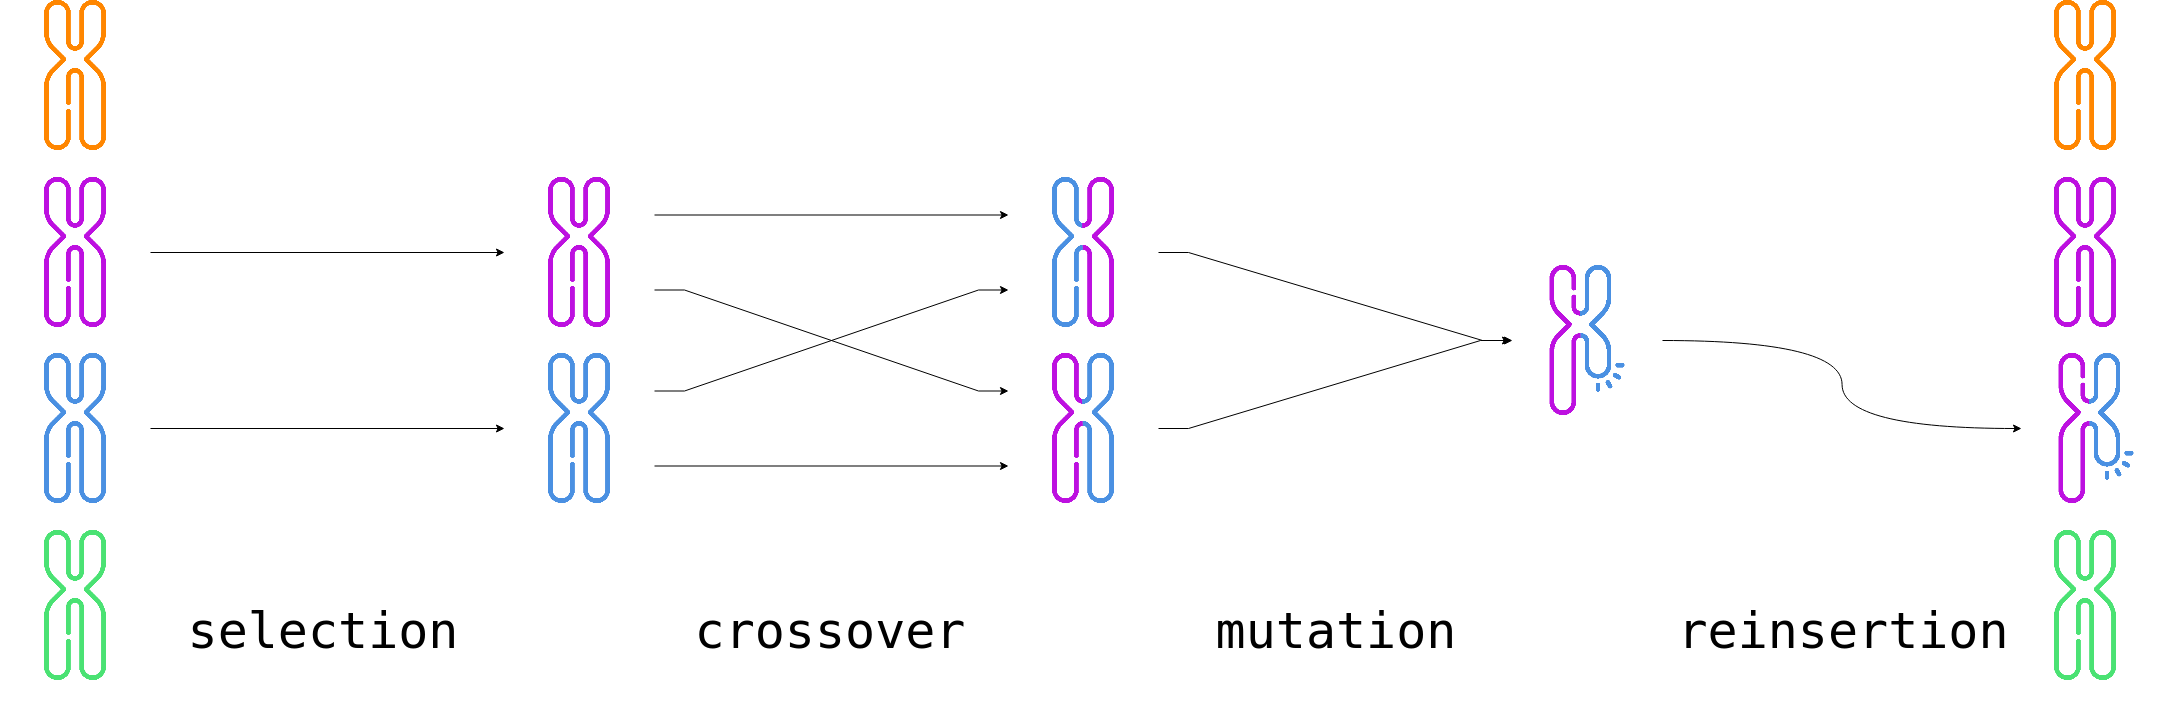
\includegraphics[width=.9\textwidth]{Images/genetic_algo.png}
\end{figure}

\subsection{Genetic Operators}

\paragraph{Tournament Selection}

Tournament selection is a strategy to select individuals for reproduction in which a subset of individuals is selected from the population and the fittest individual is chosen from the subset. Tournament selection is a generic selection operator that can be used in any genetic algorithm.

\paragraph{Mutation}

Mutation is a genetic operator used to introduce new genetic information into the population. In practice, the individual characteristic is modified by applying a random perturbation to its genetic information.

\paragraph{Elitism}

Elitism is a selection strategy in which the fittest individuals are preserved from one generation to the next. It is used to ensure that the fittest individuals are not lost during the evolution process and to speed up the convergence of the algorithm.

\paragraph{Crossover}

Crossover is a genetic operator used to combine the genetic information of two individuals to generate a new individual. In the context of evolutionary algorithms, crossover is used to generate new individuals from the population. The crossover operator is inspired by the natural reproduction process, in which the genetic information of two individuals is combined to generate a new individual. A generic \textit{k-point crossover} operator takes two individuals and a number $k$ as input and returns two new individuals. The two individuals are divided into $k+1$ segments, and the segments are then swapped between the two individuals.